% ============================================================
%  TreeFlowNet — Publication-Quality Architecture Diagram
%  Target: IEEE TGRS / ISPRS P&RS
%  Engine: pdflatex + TikZ
% ============================================================
\documentclass[tikz,border=4pt]{standalone}

\usepackage{tikz}
\usepackage{amsmath}
\usepackage{amssymb}
\usepackage{xcolor}
\usepackage{helvet}
\renewcommand{\familydefault}{\sfdefault}

\usetikzlibrary{
  arrows.meta,
  calc,
  fit,
  positioning,
  shadows.blur,
  shapes.geometric,
  shapes.multipart,
  decorations.pathreplacing,
  backgrounds,
  matrix
}

% ─────────────────────── Color Palette ───────────────────────
\definecolor{colInput}{HTML}{2A6496}
\definecolor{colBackb}{HTML}{1A4A73}
\definecolor{colFPN}{HTML}{2E7D7B}
\definecolor{colFlow}{HTML}{1B6B3A}
\definecolor{colSDT}{HTML}{6A3D9A}
\definecolor{colHeat}{HTML}{C05820}
\definecolor{colMask}{HTML}{7B5B3A}
\definecolor{colDec}{HTML}{2C3E50}
\definecolor{colOut}{HTML}{16213E}
\definecolor{colGroup1}{HTML}{EBF4FB}
\definecolor{colGroup2}{HTML}{EAF5F4}
\definecolor{colGroup3}{HTML}{F0EBF7}
\definecolor{colGroup4}{HTML}{FEF3EC}
\definecolor{colGroup5}{HTML}{EAECF0}
\definecolor{colArrow}{HTML}{444444}
\definecolor{colLoss}{HTML}{8E1F0B}

\tikzset{
  block/.style={
    rectangle, rounded corners=4pt,
    minimum width=#1, minimum height=8mm,
    align=center, font=\small\sffamily,
    draw=none, text=white,
  },
  block/.default=28mm,
  seclabel/.style={
    font=\scriptsize\sffamily\bfseries, text=#1,
    rotate=90, anchor=south
  },
  groupbox/.style={
    rectangle, rounded corners=6pt,
    fill=#1, draw=#1!60!black,
    line width=0.4pt, inner sep=5pt,
  },
  arr/.style={
    -Stealth, line width=0.9pt, color=colArrow,
    shorten >=1.5pt, shorten <=1.5pt,
  },
  skiparr/.style={
    -Stealth, dashed, line width=0.6pt, color=colArrow!60,
    shorten >=1.5pt, shorten <=1.5pt,
  },
  lossbox/.style={
    rectangle, rounded corners=3pt,
    fill=colLoss!12, draw=colLoss!40, line width=0.5pt,
    font=\tiny\sffamily, text=colLoss, align=center,
    inner sep=2pt,
  },
  note/.style={
    font=\scriptsize\itshape\sffamily, text=gray!70,
  },
}

\begin{document}
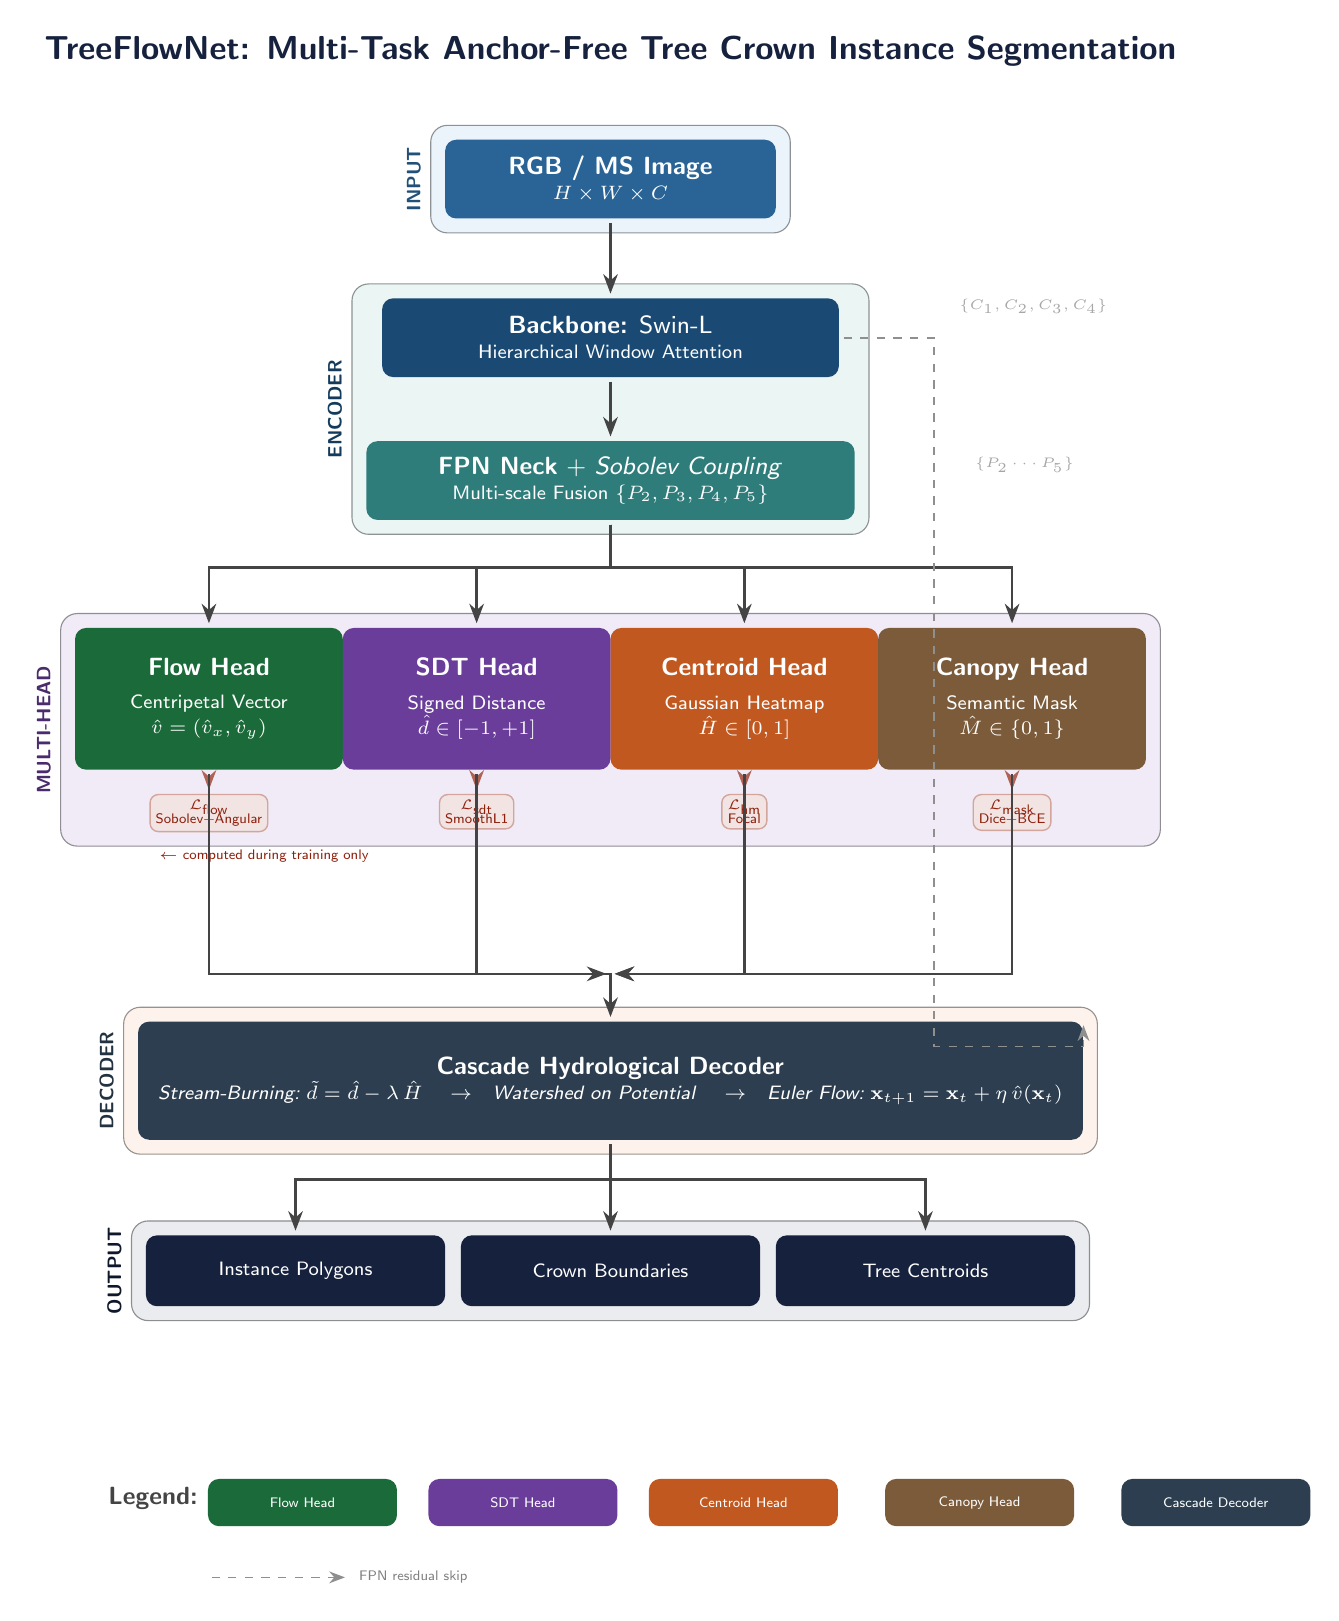
\begin{tikzpicture}[x=1mm, y=1mm, every node/.style={font=\sffamily}]

% ─────────── (A) TITLE ───────────
\node[font=\large\sffamily\bfseries, text=colOut, anchor=south]
  (title) at (0, 8)
  {TreeFlowNet: Multi-Task Anchor-Free Tree Crown Instance Segmentation};

% ─────────── (B) INPUT ───────────
\node[block=42mm, fill=colInput, minimum height=10mm, anchor=north] (inp) at (0,0)
  {\textbf{RGB / MS Image}\\[-2pt]\scriptsize $H\times W\times C$};

% ─────────── (C) BACKBONE ───────────
\node[block=58mm, fill=colBackb, minimum height=10mm,
      below=10mm of inp] (bb)
  {\textbf{Backbone:} Swin-L\\[-2pt]
   \scriptsize Hierarchical Window Attention};

% ─────────── (D) FPN NECK ───────────
\node[block=62mm, fill=colFPN, minimum height=10mm,
      below=8mm of bb] (fpn)
  {\textbf{FPN Neck} + \textit{Sobolev Coupling}\\[-2pt]
   \scriptsize Multi-scale Fusion $\{P_2,P_3,P_4,P_5\}$};

% ─────────── (E) FOUR HEADS (row, spread horizontally) ───────────

\node[block=34mm, fill=colFlow, minimum height=18mm, anchor=north]
  (hflow) at (-51mm, -62mm)
  {\textbf{Flow Head}\\[1pt]
   \scriptsize Centripetal Vector\\[-2pt]
   \scriptsize $\hat{v}=(\hat{v}_x,\hat{v}_y)$};

\node[block=34mm, fill=colSDT, minimum height=18mm, anchor=north]
  (hsdt) at (-17mm, -62mm)
  {\textbf{SDT Head}\\[1pt]
   \scriptsize Signed Distance\\[-2pt]
   \scriptsize $\hat{d}\in[-1,+1]$};

\node[block=34mm, fill=colHeat, minimum height=18mm, anchor=north]
  (hheat) at (17mm, -62mm)
  {\textbf{Centroid Head}\\[1pt]
   \scriptsize Gaussian Heatmap\\[-2pt]
   \scriptsize $\hat{H}\in[0,1]$};

\node[block=34mm, fill=colMask, minimum height=18mm, anchor=north]
  (hmask) at (51mm, -62mm)
  {\textbf{Canopy Head}\\[1pt]
   \scriptsize Semantic Mask\\[-2pt]
   \scriptsize $\hat{M}\in\{0,1\}$};

% ─────────── LOSS BOXES ───────────
\node[lossbox, below=3mm of hflow]  (lf)  {$\mathcal{L}_{\text{flow}}$\\[-1pt]\tiny Sobolev+Angular};
\node[lossbox, below=3mm of hsdt]   (ls)  {$\mathcal{L}_{\text{sdt}}$\\[-1pt]\tiny SmoothL1};
\node[lossbox, below=3mm of hheat]  (lh)  {$\mathcal{L}_{\text{hm}}$\\[-1pt]\tiny Focal};
\node[lossbox, below=3mm of hmask]  (lm)  {$\mathcal{L}_{\text{mask}}$\\[-1pt]\tiny Dice+BCE};

% ─────────── (F) CASCADE DECODER ───────────
\node[block=120mm, fill=colDec, minimum height=15mm,
      anchor=north] (dec) at (0mm, -112mm)
  {\textbf{Cascade Hydrological Decoder}\\[-2pt]
   \scriptsize
   \textit{Stream-Burning:}\;$\tilde{d}=\hat{d}-\lambda\,\hat{H}$
   \quad$\rightarrow$\quad
   \textit{Watershed on Potential}
   \quad$\rightarrow$\quad
   \textit{Euler Flow:}\;$\mathbf{x}_{t+1}=\mathbf{x}_t+\eta\,\hat{v}(\mathbf{x}_t)$};

% ─────────── (G) OUTPUTS ───────────
\node[block=38mm, fill=colOut, minimum height=9mm,
      below=12mm of dec, xshift=-40mm] (oins)
  {\scriptsize Instance Polygons};

\node[block=38mm, fill=colOut, minimum height=9mm,
      below=12mm of dec] (ocro)
  {\scriptsize Crown Boundaries};

\node[block=38mm, fill=colOut, minimum height=9mm,
      below=12mm of dec, xshift=40mm] (ocnt)
  {\scriptsize Tree Centroids};

% ─────────── GROUP BOXES ───────────
\begin{scope}[on background layer]
  \node[groupbox=colGroup1, fit=(inp),
        label={[seclabel=colInput!80!black]left:\textbf{INPUT}}] {};
  \node[groupbox=colGroup2, fit=(bb)(fpn),
        label={[seclabel=colBackb!80!black]left:\textbf{ENCODER}}] {};
  \node[groupbox=colGroup3, fit=(hflow)(hsdt)(hheat)(hmask)(lf)(ls)(lh)(lm),
        label={[seclabel=colSDT!70!black]left:\textbf{MULTI-HEAD}}] {};
  \node[groupbox=colGroup4, fit=(dec),
        label={[seclabel=colDec!80!black]left:\textbf{DECODER}}] {};
  \node[groupbox=colGroup5, fit=(oins)(ocro)(ocnt),
        label={[seclabel=colOut!70!black]left:\textbf{OUTPUT}}] {};
\end{scope}

% ─────────── ARROWS ───────────

% Input → Backbone
\draw[arr] (inp.south) -- (bb.north);

% Backbone → FPN
\draw[arr] (bb.south) -- (fpn.north);

% FPN → heads (fan-out via intermediate point)
\coordinate (fanout) at ($(fpn.south)+(0,-6mm)$);
\draw[arr] (fpn.south) -- (fanout) -| (hflow.north);
\draw[arr] (fpn.south) -- (fanout) -| (hsdt.north);
\draw[arr] (fpn.south) -- (fanout) -| (hheat.north);
\draw[arr] (fpn.south) -- (fanout) -| (hmask.north);

% Heads → losses
\draw[arr, color=colLoss!70] (hflow.south) -- (lf.north);
\draw[arr, color=colLoss!70] (hsdt.south)  -- (ls.north);
\draw[arr, color=colLoss!70] (hheat.south) -- (lh.north);
\draw[arr, color=colLoss!70] (hmask.south) -- (lm.north);

% Heads → decoder (via fan-in)
\coordinate (fanin) at ($(dec.north)+(0,6mm)$);
\draw[arr] (hflow.south) -- ++(0,-4mm) |- (fanin) -- (dec.north);
\draw[arr] (hsdt.south)  -- ++(0,-4mm) |- (fanin);
\draw[arr] (hheat.south) -- ++(0,-4mm) |- (fanin);
\draw[arr] (hmask.south) -- ++(0,-4mm) |- (fanin);

% Decoder → outputs
\coordinate (fano2) at ($(dec.south)+(0,-5mm)$);
\draw[arr] (dec.south) -- (fano2) -| (oins.north);
\draw[arr] (dec.south) -- (fano2) -- (ocro.north);
\draw[arr] (dec.south) -- (fano2) -| (ocnt.north);

% Skip: backbone → decoder (residual connection)
\draw[skiparr]
  (bb.east) -- ++(12mm,0) coordinate (skipA)
  -- ($(skipA)+(0,-90mm)$) coordinate (skipB)
  -| (dec.north east);

% ─────────── LABELS / ANNOTATIONS ───────────
\node[note, right=14mm of bb, yshift=4mm]  {\tiny $\{C_1,C_2,C_3,C_4\}$};
\node[note, right=14mm of fpn, yshift=2mm] {\tiny $\{P_2\cdots P_5\}$};

% Training-only note
\node[font=\tiny\sffamily, text=colLoss, anchor=west]
  at ($(lf.south west)+(0,-3mm)$)
  {$\leftarrow$ computed during training only};

% ─────────── LEGEND ───────────
\node[anchor=north west, font=\small\sffamily\bfseries, text=colArrow]
  (leg0) at (-65mm, -170mm) {Legend:};

\foreach \col/\lbl/\xoff in {
  colFlow/{Flow Head}/0,
  colSDT/{SDT Head}/28,
  colHeat/{Centroid Head}/56,
  colMask/{Canopy Head}/86,
  colDec/{Cascade Decoder}/116}
{
  \node[block=24mm, fill=\col, minimum height=6mm,
        anchor=west, font=\tiny\sffamily]
    at ($(leg0.east)+(\xoff mm,-0.5mm)$) {\lbl};
}

\draw[skiparr] ($(leg0.east)+(0,-10mm)$) -- ++(18mm,0)
  node[right, font=\tiny\sffamily, text=gray] {FPN residual skip};

\end{tikzpicture}
\end{document}
